\section*{Supplementary Note S8: metabolic, surface-module and viral tests of functional hypotheses}
\label{supp:mechanistic_tests}

\subsection*{Surface-associated families and the limits of context transfer}

The context screen comprised 1,460 families and six role hypotheses, giving 8,760 family-by-role tests. Candidate eligibility required independently verified loci; comparison sets included known-function exported proteins and dark proteins with verified soluble topology. The six roles were evaluated with the recorded circular-shift neighbourhood nulls. Benjamini--Hochberg adjustment used the complete test universe, including unevaluable tests assigned $p=1$ for multiplicity accounting. Genus-restricted sensitivity yielded no adjusted $q\leq0.10$ association (minimum $q=1$). The genome-level associations are therefore interpreted alongside the observed local synteny and their lineage dependence.

Family \texttt{22PRr1::\allowbreak22PRr1\_2531955\_3} had 13 independently verified adjacent, co-oriented pairs across six genus-or-singleton groups, with gaps from $-4$ to 37~bp (negative values denote overlap). Its partner belongs to dark family F37Dr2 and carries the bacterial PilJ-family profile PF04964. The surveyed five-gene windows on either side lacked annotated core archaeal pilin machinery; genome-wide machinery status remains unresolved. The family's genome-level joint $q$ was 0.0021. The available seed model yielded a maximum query TM-score of 0.2898 against the tested archaeal pilin/archaellin references. The verified interior representative, \texttt{1PRr2\_\_self\_SemiBin\_81::\allowbreak1PRr2\_468829\_3}, had no model available.

Family \texttt{V60PRr2::\allowbreak V60PRr2\_1314979\_4} had 11 independently verified adjacent, co-oriented pairs across five genus-or-singleton groups, with gaps from $-4$ to 6~bp. Its partner carried PF18204/PF10731 profiles and a structural relationship to a cell-surface glycoprotein reference. Its genome-level joint $q$ was 0.00035. The candidate seed had no qualifying match to the tested surface-layer panel; its verified interior representative, \texttt{V47PRr1\_\_self\_SemiBin\_699\_sub::\allowbreak V47PRr1\_105096\_18}, had no model available. Partner annotations describe the neighbouring protein and provide a context hypothesis for the candidate.

The 47-family follow-up audited 428 loci, of which 326 were complete interior coding sequences. Exact-sequence structural models were available for 32 loci, including 27 complete interior loci. Alignments were completed for 29 families; 18 remained unevaluable under the sequence-admission rules. Across the full 1,460-family screen, 565 seed models matched the query sequence, 802 models were unavailable and 93 mismatched the query. Missing and mismatched models were excluded from structural evidence. Curated reference self-searches and confusable-chain controls checked search recovery and chain identity. The final dispositions were 38 families with insufficient evidence and nine with exploratory fold or motif hypotheses lacking convergent operon evidence. The GSPA component re-evaluated the frozen three-genome pilot; training-set provenance and graph leakage remained unresolved, so these predictions retained exploratory status.

\subsection*{Metabolic-model sensitivity and masked-gene recovery}

We evaluated gapseq-derived networks for 237 desert and 247 external genomes, retaining the latter's 218 GTDB and 29 MGnify origins. The candidate pool contained 2,271 observed reactions from cohort draft and gap-filled models. One elementally imbalanced reaction was excluded; reactions with unresolved formula or charge retained explicit status. The archaeal biomass template derives from \emph{Methanosarcina barkeri}. We compared this baseline with component-omission recipes, including removal of seven non-$F_{420}$ trace cofactors while retaining $F_{420}$. Media ranged from fixed oxic and anoxic hydrogen/carbon-dioxide/ammonium recipes to organic-acid, amino-acid and precursor-containing recipes. These are declared model scenarios rather than measured soil media.

Across 12,580 evaluated genome--medium--biomass cases, 10,578 yielded verified feasible ensembles, 1,936 were infeasible under the fixed medium, and 66 remained numerically unresolved (56 flux-verification failures and ten timeouts without a feasible incumbent). Four optional native-medium cases were unavailable because their media were empty. Binary mixed-integer optimisation enumerated alternative additions within 25\% of the weighted-cost bound, with a six-second limit per solve and closed-uptake energy-cycle checks. Reported reaction counts are the smallest among found valid solutions; global optimality was unproven. Raw flux vectors were not retained, and the package distinguishes verification of the stored solution ledger from a fresh flux replay.

For the anoxic organic-acid and amino-acid medium, 236 desert genomes had evaluable paired baseline and seven-cofactor-omission solutions. The median decrease in added-reaction count was 73 (interquartile range 70--76), with 213 decreases and 23 increases. Weighted costs and alternative solutions allow reaction counts to increase even when biomass requirements are relaxed. Between-cohort comparisons were descriptive, with separate accounting for quality-estimation methods and shared taxonomic orders.

To assess recovery rather than feasibility alone, we masked 10\%, 20\% or 30\% of genes, with three replicates per level, in seven reference genomes meeting numerical completeness $\geq90\%$ and contamination $\leq5\%$. This selection did not require the rRNA and tRNA evidence used for formal MIMAG high-quality classification. All masked runs used the same oxic organic-acid and amino-acid medium and seven-cofactor-omission biomass as their unmasked baselines. Averaging first within each genome and then across the seven genomes, recovery of masked gene-associated reactions was 16.8\%, whereas alternative reactions constituted 76.7\% of newly induced additions. The model ensembles and assembly-level homology checks provide conditional pathway hypotheses; specific enzyme assignments and exchange between community members remain unresolved.

\subsection*{Complete microTrait profiles and metabolic context}

The shared resource provides microTrait profiles for the same 5,438 canonical genomes, including all 237 Thermoplasmatota, as \texttt{EQ-MICROTRAIT-\allowbreak REP-\allowbreak v1.0.0} \citep{rubalkhali_datapaper,karaoz2022microtrait}. These profiles use fresh Prodigal v2.6.3 calls in metagenomic mode, independently of the earlier Pyrodigal and KO analyses. We interpreted a positive aggregated category as at least one satisfied constituent rule. We retained the complete rule definitions, per-genome outputs, canonical taxonomic joins and a numerical quality sensitivity (completeness $\geq90\%$, contamination $\leq5\%$). The category ``protein degradation'' includes intracellular peptidases, proteasome components and processing enzymes, so category positivity supports a broad protein-processing capacity. Extracellular degradation requires localisation and substrate evidence for the individual proteins.

\begin{table}[htbp]\centering\small
\caption{Thermoplasmatota with positive microTrait rule categories. Entries are genome counts, with the denominator shown in each column. The quality sensitivity is a numerical completeness/contamination filter; formal MIMAG high-quality status has additional criteria.}
\label{tab:microtrait_thermo}
\begin{tabular}{lrr}\toprule
Category & All genomes ($n=237$) & Quality subset ($n=59$)\\\midrule
Free-amino-acid transport & 237 & 59\\
Peptide transport & 10 & 1\\
Protein degradation/processing & 237 & 59\\
Carbon-fixation marker category & 2 & 1\\\bottomrule
\end{tabular}
\end{table}

The two positive carbon-fixation calls arose from the microTrait 3-hydroxypropionate/4-hydroxybutyrate marker rule. This rule admits alternative subsets of reactions; the earlier KEGG module analysis required at least two-thirds module coverage and recovered neither of the two canonical archaeal fixation cycles shown in Fig.~\ref{fig:ecology}c. These endpoints measure different levels of pathway evidence. The rule-level calls remain candidates for pathway inspection, while autotrophic growth remains unresolved. Growth and optimum-temperature predictions are distributed with applicability flags and were not used to infer in situ growth rates or to replace the separate gRodon2 ecological analysis.

\subsection*{Sequence-qualified archaeal host--virus candidates}

We screened all 591 archaeal representatives for CRISPR arrays and resolved spacer matches against exact viral target sequences, retaining genome identifiers, target checksums and viral-boundary evidence. Of these genomes, 144 had recovered spacers and 447 were untested by spacer matching. After removing an alias duplicate and unresolved or boundary-sensitive assignments, the primary set contained five candidate pairs across four archaeal hosts. One involved Thermoplasmatota host \texttt{41PRr2\_\_single\_SemiBin\_236}. Its array-bearing contig had corroborative archaeal-associated coding context; the host taxonomy remains conditional on MAG bin membership. A second Thermoplasmatota candidate was retained separately: its matching interval lay outside the catalogue viral core but within a longer CheckV viral interval, leaving viral ownership of that extension unresolved.

Competitive read mapping covered 14 selected libraries and retained separate raw-read and MAPQ~20 summaries. Only one viral sequence--sample combination met the primary population-profiling gate. The supplementary inStrain audit distinguished one-read breadth from depth-qualified breadth (at least five reads), verified terminal completion, and separated cryptic variant sites from exported variant calls. The host-association models had sparse outcomes, missing covariates and rank deficiency; the overparameterised adjusted model was not fitted. Family and abundance comparisons remain exploratory. The spacer links identify historical-exposure candidates, while active infection, host preference and a causal role for the dark proteins remain unresolved.

\subsection*{Eligibility of an independent soil proteogenomic dataset}

We evaluated the soil-warming proteogenomic dataset of Karaoz and colleagues \citep{karaoz2026proteogenomics} for independent support of the two surface-associated leads. The dataset contains 30 samples nested within three heated--control plot pairs and five depths. Its 113 dereplicated archaeal genomes include 38 Thermoplasmatota, but none from the focal class SW-10-69-26. Searches used all admitted family sequences, genetic-code-aware translations and uncapped sequence/profile searches. Peptide-spectrum matches required both the reported peptide and spectrum $q$-values to be at most 0.01, with peptide specificity checked against the available sequence background and shared spectra counted once.

None of the 15 split FASTAs constituting the full search database was available among the deposited files. Consequently, global peptide uniqueness and full search-database inclusion could be checked only for a subset of sequences. Neither lead obtained independently evaluable family-level expression validation. One broader exported-dark family had provisional support from five peptides and six spectra within the observed subset, attributable to Nitrososphaeraceae homologues; this remains separate from the focal Thermoplasmatota leads. The package retains observed-subset detections, absent study-genome homologues and unverified search inclusion as distinct outcomes. Primary family-level warming responses remain non-estimable; the three plot pairs are the independent experimental units.

\begin{figure}[p]\centering
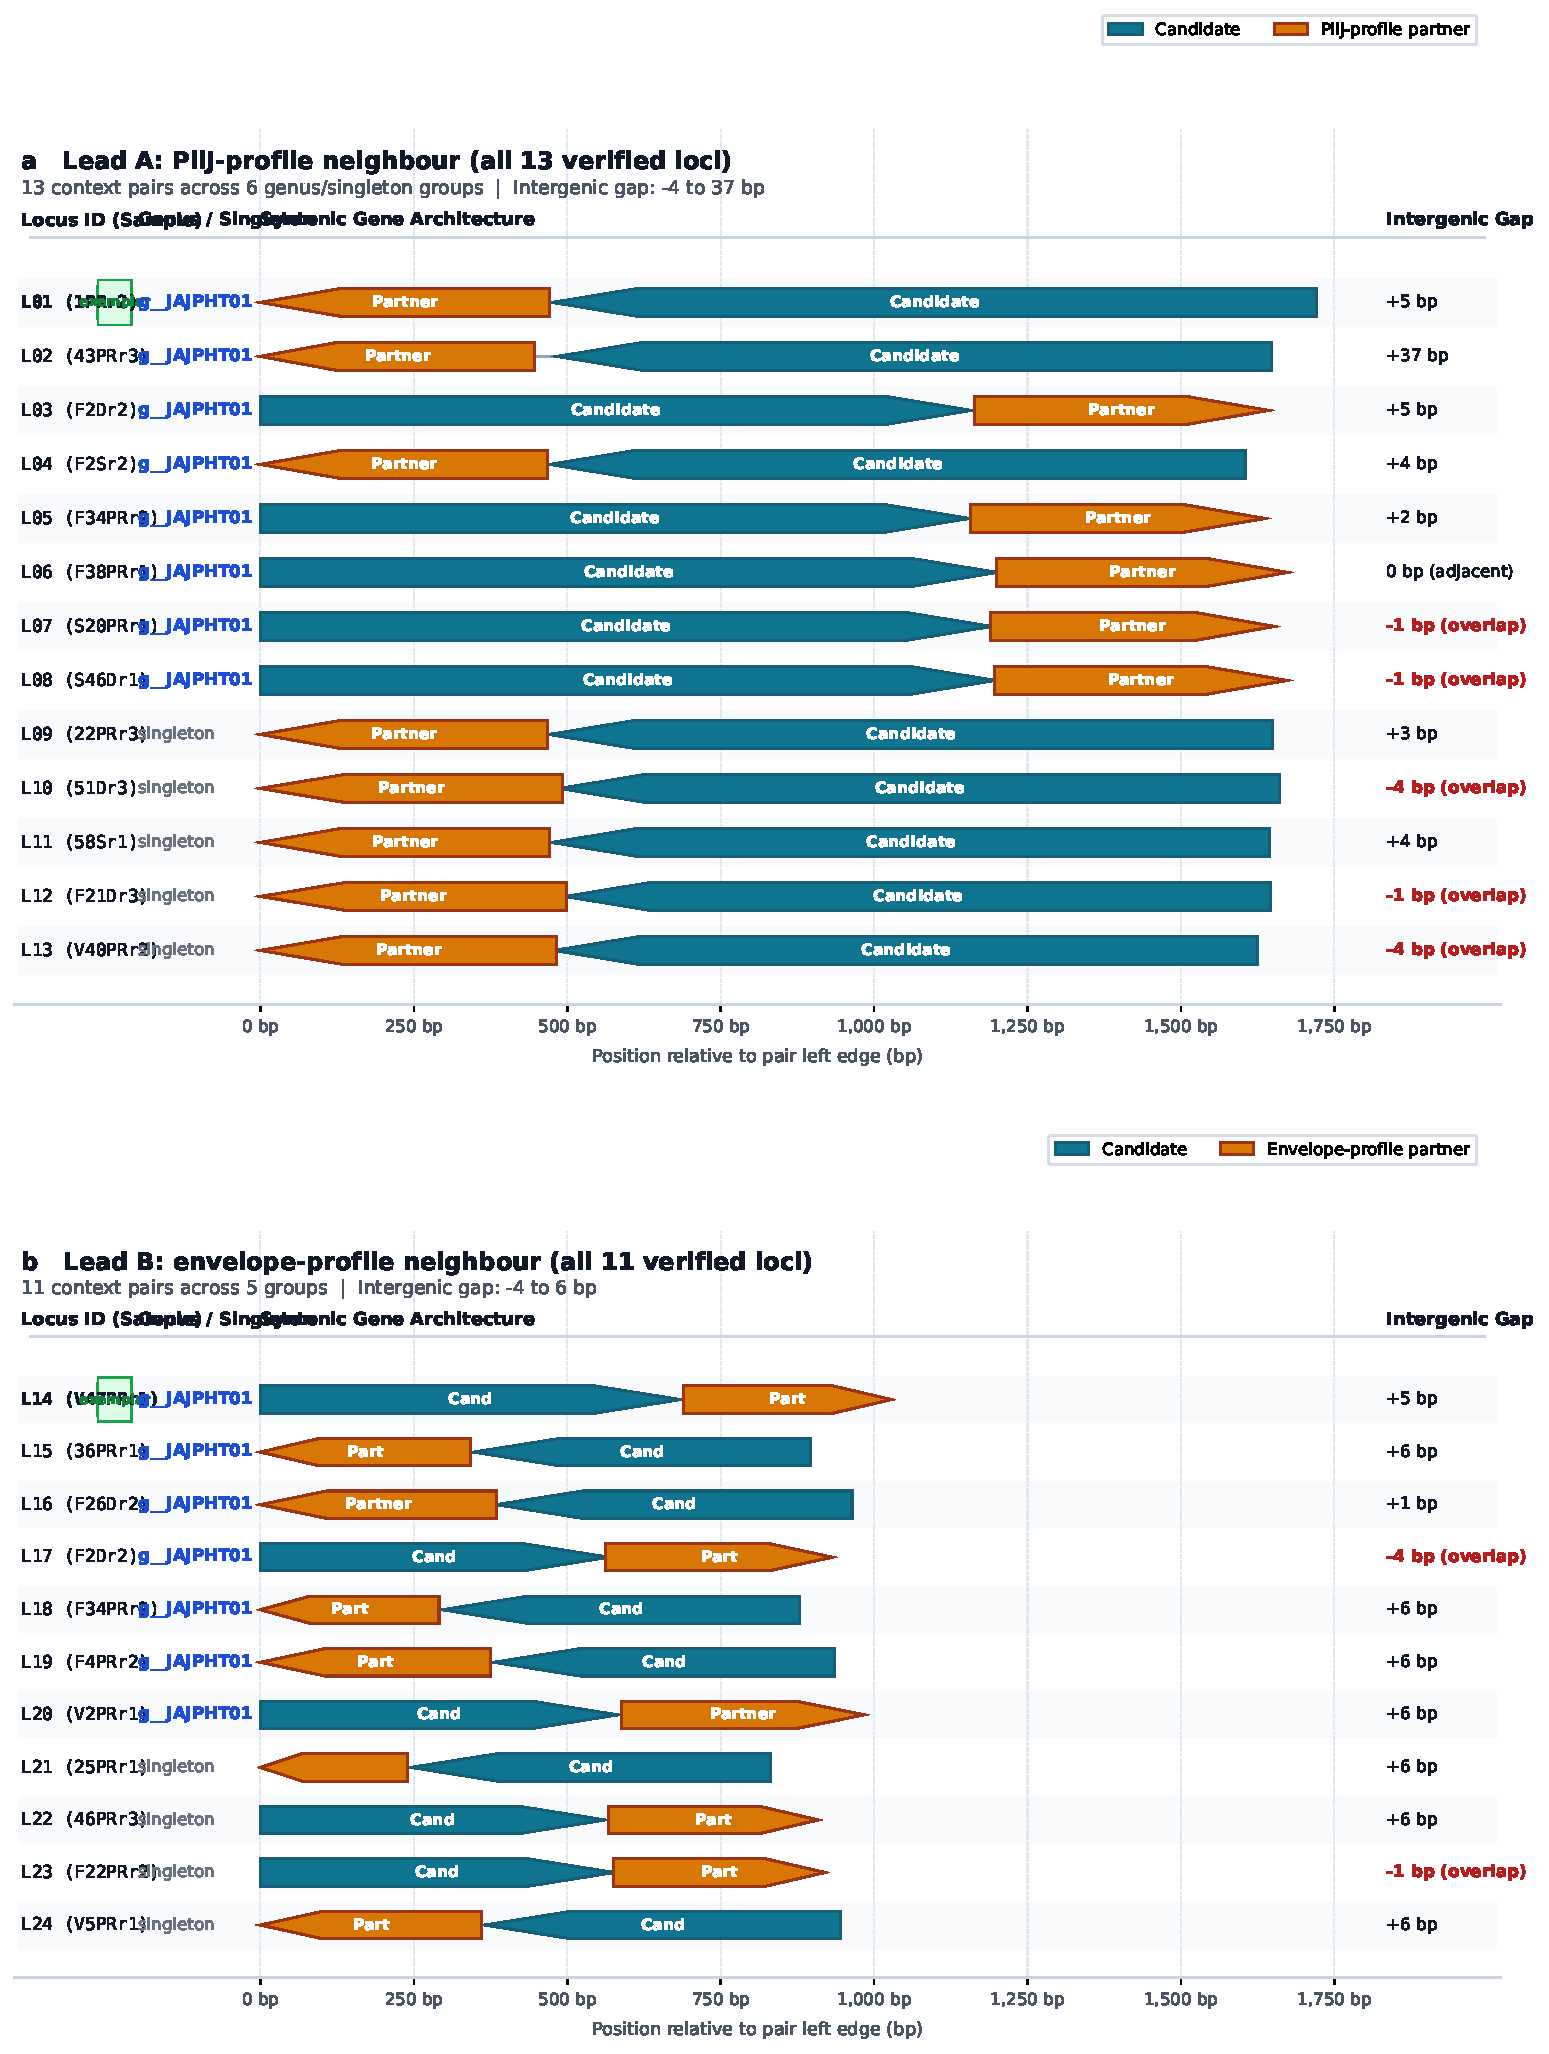
\includegraphics[width=\textwidth,height=0.79\textheight,keepaspectratio]{figures/fig_surface_modules_all_loci.pdf}
\caption{All verified contexts for the two surface-associated leads. Arrows retain native strand orientation and verified nucleotide lengths; coordinates start at the left edge of each pair. Negative intergenic gaps denote overlaps. Locus identifiers resolve to full genome and gene identifiers in the source table. The 24 pairs comprise 13 contexts for lead A and 11 for lead B, all adjacent and co-oriented. Genus-or-singleton labels distinguish named genera from genomes lacking a genus assignment.}
\label{fig:surface_all_loci}
\end{figure}
